\chapter{Design of Experiments}
\chaptermark{DOE}
\label{ch:doe}


This chapter is devoted to the matter of designing studies, and follows the lines of \cite{cox_theory_2000} and \cite{cox_principles_2011}.
As we will see, empirical studies come in many forms and shapes. 
The most fundamental distinction is between \emph{observational studies} and \emph{designed experiments}.\marginnote{Observational Studies}
This distinction is performed along our ability to control the studied effects, and will have crucial implications on the interpretation of results, and in particular, on causality claims. 




\section{Challenges in Empirical Studies}

The challenges in all empirical studies, be it designed experiments, or observational are:
\begin{description}
	\item [Systematic errors] 
	Can be thought of as bias, even thought much more general than the narrow definition in statistical theory. 
	Refers to the distortion of conclusions due to confusion sources that do not cancel out in the long run. 
	\item [Non-systematics errors]
	Can be thought of as the ``noise''. 
	If the non-systematic errors are large, then noise may mask the signal. 
	\item [Uncertainty in conclusions]
	Only in the formalism of mathematics and logic things are true or false with certainty. 
	In natural sciences we have assumptions, and confidence levels.
	Each conclusions should thus be accompanied by the level of certainty in which it is stated. 	
	\item [Efficiency]
	The above goals may certainly be achieved given unlimited resources. 
	Achieving them quickly and cheaply, is a worthy goal, and a veritable art. 	
	\item [Range of validity]
	Do our conclusions hold in all countries? Weathers? Altitudes? Races? 
	How general are our conclusions? 	
\end{description}



\subsection{Dealing with Systematic Errors}

Systematic errors arise from two sources: either the study design is such that it does not measure what we think it measures, or leakage of personal judgment.

The first source of systematic errors can be dealt at the design stage, or at the analysis stage.
Much emphasis is given in the literature to unbiased estimation, but reality is that a good design can save a lot of trouble at the analysis stage. 
Later in this chapter, we will discuss in detail the means to avoid systematic errors. 


\subsection{Dealing with Non-Systematic Errors}

Informally speaking, non-systematic errors are avoided by:
\begin{description}
	\item [Compare like with like] Comparing similar units. Put differently, we aim to compare like with like. 
	This is done by the sampling scheme. 
	\item [Replications] 
	Repeat a measurement enough times, and the non-systematic error will cancel out. 
\end{description} 




\subsection{Sampling}

The literature of sampling is divided between method for sampling in designed experiments, and sampling in observational studies. 
In both cases, we will typically want sampling schemes that reduce the 



\subsubsection{Non-simple sampling}
Throughout this chapter we will be considering simple random samples, where all the population units have the same probability of being sampled. 
For completeness, we will emphasize that this is not always the case as illustrated in the next example.

\begin{example}[Respondent Driven Sampling]
	\label{ex:RDS}
	Consider the following chain-referral sampling scheme. 
	A Facebook questionnaire is passed by rewarding respondents some credit if they name other respondents.
	The probability of being sampled is thus not fixed for everyone, but rather a function of the number of your facebook friends.  
	Now imagine the questionnaire is meant to estimate the market share of product Y.
	It seems reasonable to assume that the more friends you have, the more likely you are to be sampled, and also, the more likely to be familiar with Y. 
	This sampling scheme will thus lead to an upward biased estimate of Y's popularity.
\end{example}

If the non-simple sampling scheme in Example~\ref{ex:RDS} is not accounted for at the analysis stage, we will clearly have biased popularity estimates. 
To deal with over-representation we will want to weight each sample by its probability of being sampled.
\begin{definition}[Horowitz Thompson Estimator]
	\label{def:horowitz-thompson}
	If each unit $i$ has probability $\pi_i$ of being sampled and measured response $y_i$, then an unbiased estimate of the population mean of $y$ is given by 
	\begin{align}
	\frac{\sum_{i \in S} y_i/\pi_i}{\sum_{i \in S} 1/\pi_i},
	\end{align}
	where $i \in S$ means that $i$ has actually been sampled. 
\end{definition}
You may verify that the Horowitz-Thompson estimator in Definition~\ref{def:horowitz-thompson} return the usual sample mean, if the sampling is simple, thus all $\pi_i$ are equal. 
From this point on, we ignore special sampling schemes and return to simple random sampling. 





\section{DOE Preliminaries}
\label{sec:DOE_preliminaries}

We will now discuss \emph{designed experiments}. 
Observational studies are briefly discussed in Section~\ref{sec:observational}.

When designing a product (remember DFSS \ref{sec:dfss}), or once a control chart has signaled an alert, we will want to know what \emph{controllable inputs} influenced our process, and how to reduce its variability.
In our SPC terminology, we will want to know what are the \emph{causal effects} of our controllable inputs (\emph{factors}), on our \emph{CTQ} (\emph{response}). 
The theory of discovering these effects is the theory of \emph{design of experiments} (DOE).
Its goal is to compare the response under various conditions in order to \emph{screen} factors with no effect, 
to \emph{estimate} effect sizes, 
find \emph{optimal} factor-level combinations, 
and remove assignable variability; 
all these as \emph{efficiently} as possibly.


Several matters should be emphasized:
\begin{description}

\item [Randomization] is the random assignment of units to treatments. 
It is fundamental to our purpose because the idea of an \emph{effect} implies \emph{causality}. 
Since we seek to intervene in the production to reduce variability, we only care about causal effects. 
It is the mechanism of \emph{randomization}, that allows us to conclude that the correlations we find are indeed causal, and not merely statistical.
For a treatment of causal inference in non-randomized experiments, i.e. in \emph{observational data}, see for example \cite{rosenbaum_observational_2002}.

\item [Pre-experiment] In this text we take it for granted that the purpose of the experiment is well known, and the candidate factors defined. 
We are fully aware, as should be the reader, that in application this is a non-trivial luxury. 
Indeed, a lot of meetings, planning, and expertise go into the selection of factors, their candidate levels, etc.

\item [Power Analysis] Part of the pre-experiment may include a power analysis. 
The pre-experiment power analysis will typically be very approximate, and rely on many assumptions. 
It is still important, as it gives an idea of the feasibility of an experiment, and avoids wasting resources.

\item [No Textbook Solution] We will present many design ideas and principles, yet in real life problems rarely obey text-books.
You should thus feel free, and even obliged, to think about your particular problem and adapt the experiment as you best see fit. 

\item[Data Analysis]
In this text, we only discuss the \textbf{design} of the experiment, and not the \textbf{analysis} of the data.
This is a non-standard choice as DOE is typically presented alongside the \emph{analysis of variance} (ANOVA) framework. \marginnote{ANOVA}
We decouple the two for several reasons. 
First, because \cite{cox_theory_2000} do so. 
Second, because these are two different thing.
The ANOVA framework may be replaced by the framework of \emph{linear models}, \emph{mixed models}, \emph{variance components}, and possibly others analysis frameworks. 
There is a vast literature focusing on the analysis.
If asked, this author may recommend \cite{hocking_analysis_1985}, which presents both the ANOVA terminology, and the linear models terminology.

\end{description}


We start by establishing DOE terminology. 


\subsection{Terminology}
Many, if not most of the following terms, originate in R.A. Fisher's seminal book ``The Design of Experiments'' \citep{fisher_design_1960}. 
As such, the DOE literature is rich in agricultural terms, due to its historical origins.
When old ideas get new names, we try to emphasize this in the text.


\begin{tcolorbox}[breakable]
\begin{description}

\item [Design]  Complete specification of experimental test runs, including blocking, randomization, repeat tests, replication, and the assignment of factor–level combinations to experimental units.

\item [Experimental Unit]  Entity on which a measurement or an observation is made.

\item [Homogenous Experimental Unit] Units that are as uniform as possible on all characteristics that could affect the response.

\item [Factors]  A controllable experimental variable that is thought to influence the response. 
In the language of SPC: \emph{a controllable input}.

\item [Level] Specific value of a factor.

\item[Treatment] The particular factor-level combination applied to an experimental unit. 
\Aka \emph{manipulation}, or \emph{cell}.

\item [Factor Encodings] 
The numerical encoding of factor levels.
Of minor importance for designing. 
Of major importance for analysis.
Two level factor encodings include:
	\begin{enumerate}
	\item Effect coding: where levels are encoded with $\set{-1,1}$.
	\item Dummy coding: where levels are encoded with $\set{0,1}$.
	\end{enumerate}

\item [Design Matrix] A matrix description of an experiment that is useful for constructing and analyzing experiments.

\item [Response] 
The CTQ in the SPC literature. 
The $y$ variable in the regression literature. 
The \emph{response} in the DOE literature. 

\item [Main Effect] Change in the expected response between two factor–levels.  
We emphasize that effects, unlike simple population parameters, imply a causal relationship.
Akin to the \emph{assignable causes} in the SPC literature, and $\beta$'s in the regression literature. 

\item [Interaction] Existence of joint factor effects in which the effect of each factor depends on the levels of the other factors.
Part of the \emph{assignable causes} in the SPC literature.

\item [Noise] \Aka \emph{error}. 
The variability in the response that cannot be attributed to any factor.
This is the \emph{common} variability in the SPC literature, and the $\varepsilon$ in the regression literature. 

\item [Replication] A single repetition of an entire experiment, i.e., a single measurement of the response in all experimental conditions.

\item [Repeats] Repeated measurements on the response under the same conditions, i.e., under the same treatment. \Aka \emph{repeat tests}.

\item [Covariate]  An variable that influences the response but is unaffected by any other experimental factors.
We cannot change at will, but we can \emph{control/account for them}. 

\item [Non Specific Factor] A variable that we suspect to affect the response, but we can only vaguely define, thus impossible to measure. 
As a consequence, we will not care to study its effect, but rather just remove it (e.g. by blocking). 
Think of ``life style'' as an example of a non-specific factor.

\item [Blocking]  Blocking, or \emph{grouping}, is an experimental design technique that removes excess variation by grouping experimental units or test runs so that those units or test runs within a block are more homogeneous than those in different blocks. Blocking attributes are also known as \emph{non specific factors}.
The blocking in the design needs to be accounted at the time of the data analysis.

\item [Confounding] When the design is such that several effects cannot be told apart. \Aka \emph{aliasing}.

\end{description}

\end{tcolorbox}











\section{Systematic Errors in Designed Experiments}

Dealing with systematic errors is possibly the greatest concern in causal inference. 
Be it a medical intervention, an industrial production process, an economic policy, or a social welfare plan- all of these critically rely on a fair assessment of the magnitude of the effect of the intervention. Bias is disastrous. 

Bias originates from two sources.
The first is some unwelcome property of the data collecting process. 
The second is by the leakage of some personal judgment into the measuring or analysis. 

\begin{example}[Judgment leaking into measurements]
	Consider cancer patients assigning themselves to the treatment or placebo groups. 
	This \emph{self selection} will clearly bias the reported effect of the new drug (who would willingly choose the placebo?!?). \marginnote{Self Selection}
\end{example}


\begin{example}[Judgment leaking into analysis]
	Return to the new-drug experiment. 
	This time, imagine the data analysis, an employee of the pharmaceutical company, known that ``Drug A'' is the new drug his company has been working on, which will grant him a considerable bonus if marketed. 
	Can he be expected to perform a fair analysis?
\end{example}

Two ways to deal with such bias:
\begin{description}
	\item [Balanced Design]
	In the simplest interpretation of ``balance'' we mean a design where an equal number of units is assigned to each treatment.
	More generally, we will keep ``balance'' by \emph{randomization}, and implying some symmetry in the combinatorial design of the experiment. 
	
	\item [Bliding]
	By blinding we mean that personnel is unaware of the factors being studied. 
	In regular blinding, subject are unaware of the treatment they are being administered. 
	In \emph{double blinding}, the experimenters and analysis are unaware of the treatments they are studying. 	 
	
\end{description}







\subsection{Non Systematic Errors in DOE}
\label{sec:variance_components}
%TODO: relate to imptoving precision in sampling. 


The idea that random samples come with (common causes of) variability, i.e. noise, should not be new to the reader.
In this section, we will try to decompose variability into it sources, and learn several techniques to reduce them. 
Starting with a motivating example, which you should use to fix ideas as you progress along this chapter. 



\begin{example}[Web Design]
\label{eg:web_design}
Consider the problem of optimizing a web site, where individuals performance is measured by conversion rate (the probability of a new user to signup, purchase, etc).
In the DOE language, the conversion is the \emph{response}.
A user (or ip address) is an \emph{experimental unit}.
The site's attributes are the \emph{factors}.
A particular site's design, i.e. a combination of factors, is the \emph{treatment}.
The users' attributes are \emph{covariates}. 
The user's life-style, a \emph{non-specific factor}.
If the site's attributes affect differently users with different attributes, we say there is an \emph{interaction}.
\end{example}




\begin{example}[Two Competing Diets]
\label{eg:diets}
Consider the problem of comparing two nutrition diets. 
Clearly, the effect of a diet on life expectancy strongly interacts with both genetics and life style. 
It would be thus very nice if we could block experimental units, so that each block has a homogenous genetics and life-style. 
That is why \textbf{twins} are so popular when designing experiments!
\end{example}







%TODO: update guage R&R experiments from Cox.
\subsection{Gage R\&R Studies}
R\&R stands for \emph{repeatability} and \emph{reproducibility}.
These experiments are aimed at assessing the irreducible non-systematic errors in measurement and \emph{range of validity} of conclusions.
As such, in a typical gauge R\&R experiment, measurement will be made under the same conditions in different labs, by different technicians, etc. 






\subsection{Completely Randomized Designs}
In the simplest of designs, all experimental units are randomly assigned to treatments. 
This is typically easy to implement.
In Example~\ref{eg:web_design} this would imply randomly assigning users to interfaces.
In Example~\ref{eg:diets} this would mean ignoring the fact that the experimental units come in naturally blocked groups of two, and randomly assigning all people to treatments. 
If you suspect, as you should, that in both examples we may reduce variability by grouping units together, keep reading.






\subsection{Randomized Block Designs}
The idea of \emph{blocking} is to replace the complete randomization scheme by a restricted randomization scheme so that variability can be reduced without introducing bias. 
The restricted randomization is created by \emph{grouping}, or \emph{blocking} groups of experimental units, and randomizing allocation within the group. 

In the twins example, nature has provided us with natural blocks of two. 
If comparing two treatments, we would naturally randomize treatments within twin-pair. 
This is known as a \emph{randomized complete block design}. \marginnote{Complete Block Design}
If we had three treatments, or more, to compare, we cannot completely randomize. This is knows as an \emph{incomplete block design}. 
There are several approaches to incomplete block designs, but we refer the reader to \cite[Sec.4.2]{cox_theory_2000} for details.

\begin{remark}[Paired sample]
While we try to avoid matter of data-analysis, it should be obvious to the reader that a two-group randomized block design should be analyzed as a \textbf{paired sample}. 
\end{remark}

In our web-design example nature has not provided natural homogenous blocks, but we can create them ourselves. 
We could block individuals along, say, the age covariate. 
We would then randomly assign users to layouts, only \textbf{within} age groups, so that all layouts are presented to each age-group. 
If each age group has as many users as there are different site designs, this is a randomized complete block design. 
If there are more layouts than users per age group, this is an incomplete block design. 
Another idea is to use each user as his own block, by introducing a temporal dimension to the experiment.
We could show all layouts to the same person. 
This particular type of blocking is known as a \emph{crossover} design, discussed in Section~\ref{sec:crossover}.

In summary, blocking is done in order to create homogeneous groups. 
Put differently: compare like-with-like. 
One can block in along factors, covariates, or non-specific factors. 
One can then compare treatments only within blocks (e.g. the paired sample t-test), thus gaining accuracy by avoiding the variability between blocks. 
A good blocking strategy is such where blocks are very homogenous within themselves, but very different between themselves, at least with respect to the response being studied. 


\begin{think}
With twins, you can have a complete block design comparing only two treatments. 
How would you go about to compare $3$ treatments?
And $k>2$ treatments?
\end{think}






\subsubsection{Crossover Design}
\label{sec:crossover}

Return to the diet comparison of Example~\ref{eg:diets}. 
Now assume that $5$ diets are being compared, and requiring quintuplets\footnote{Five identical siblings.} will severely limit the available sample size. 
If the response of different people to the diets is strongly affected by genetics \andor lifestyle, it may be the case that by (randomly) assigning diets to individuals the diets effect will be completely masked by the variability between subjects. 
To solve this, we could give each subject all $5$ diets. 
Each subject would act as his own block.
Diet effect would be analyzed within subjects, and hopefully, having removed the variability between subjects, the diet effect would reveal itself. 

Enter a new complication. 
What if the response to a particular diet is affected by the previous diet?
This is known as a \emph{carryover effect}, or \emph{residual effect}, which may bias the main layout effects of interest. \marginnote{Carryover Effect}
If all subject receive diet B after A, then the estimated effect of B will be biased by the carryover effect of A. 
A way to ``average out'' this carryover effect is to balance the treatment sequences. 
If each subject is randomly assigned to one of the $5!$ diet arrangements this balance would be achieved.

The idea of administering all treatments to each unit, in a random sequence that balances carryover effects is known as a \emph{fully randomized crossover design}. \marginnote{Fully Randomized Crossover}
Table~\ref{tab:crossover} demonstrates the $3!=6$ sequences for a $3$ treatment problem.
\begin{table}[ht]
\centering
\begin{tabular}{rlll}
  \hline
 & 1 & 2 & 3 \\ 
  \hline
1 & 1 & 2 & 3 \\ 
  2 & 2 & 3 & 1 \\ 
  3 & 3 & 1 & 2 \\ 
  4 & 1 & 3 & 2 \\ 
  5 & 2 & 1 & 3 \\ 
  6 & 3 & 2 & 1 \\ 
   \hline
\end{tabular}
\caption[Crossover Design]{Crossover design: a balanced sequence of administration of $3$ treatments, generated with the \rcode{des.MOLS()} function of the \rcode{crossdes} \R package. }
\label{tab:crossover}
\end{table}









\section{Efficiency in Design-- Factorial Designs}
\label{sec:factorial_design}

In the previous section we discussed methods of reducing the variability in the response to each treatment, so that we can better reveal differences between treatments. 
In the current section we will break treatments into smaller building blocks; \emph{factors}.
By doing so we will gain efficiency. 
Each sample will give us information on the effect of various \emph{factors}.
We will also be able to learn if the effect of factors are additive, or non additive, and we will be able to extrapolate from observed treatments, to unobserved treatments. 


\begin{example}[Web design revisited]
\label{eg:web_design_II}
Back to the web-design from Example~\ref{eg:web_design}, assume now that treatments, i.e. layouts, differ in the location of a button, the colour of the heading and the size of the logo. 
If each has two possible levels, we deal with $3$ factors with $2$ levels each, totalling in $8$ different layouts. 
Instead of estimating the effect of the $8$ layouts, we estimate the effect of each of the $3$ factors. 
Given a budget of, say, $n=8$ observations, we would have one observation per treatment. 
The magic of a factorial design is that we have $4$ observations for each factor level.
If we treat a web-design as the sum of its factor effects, we have gained accuracy 
\end{example}

\begin{think}
Is the magic of the factorial design a free lunch? 
No. The lunch has a price.
The price is that we have assumed that a site is the sum of its components, without interactions. 
Without this assumption, there is nothing to gain from a factorial design.
\end{think}








\subsection{Full Factorial Designs}
A \emph{full factorial}, or \emph{complete factorial} design, is one where all factor-level combinations are replicated the same number of times.
The most common of the full-factorial designs is the $2^k$-design where all combinations of $k$ factors with two levels each are tested in each replication.



\subsubsection{$2^k$ design}
Consider two factors denoted $A$ and $B$.
Adopt the effect coding so that we encode their levels by $\set{-1,1}$.
The design matrix of a single replication is depicted in Figure~\ref{fig:full_factorial} (top right) along with a visualization of the design (top left).
Allowing $n$ observations per condition, the experiment will include $4n$ observations, which will be randomized between conditions.

\begin{figure}[H]
\centering
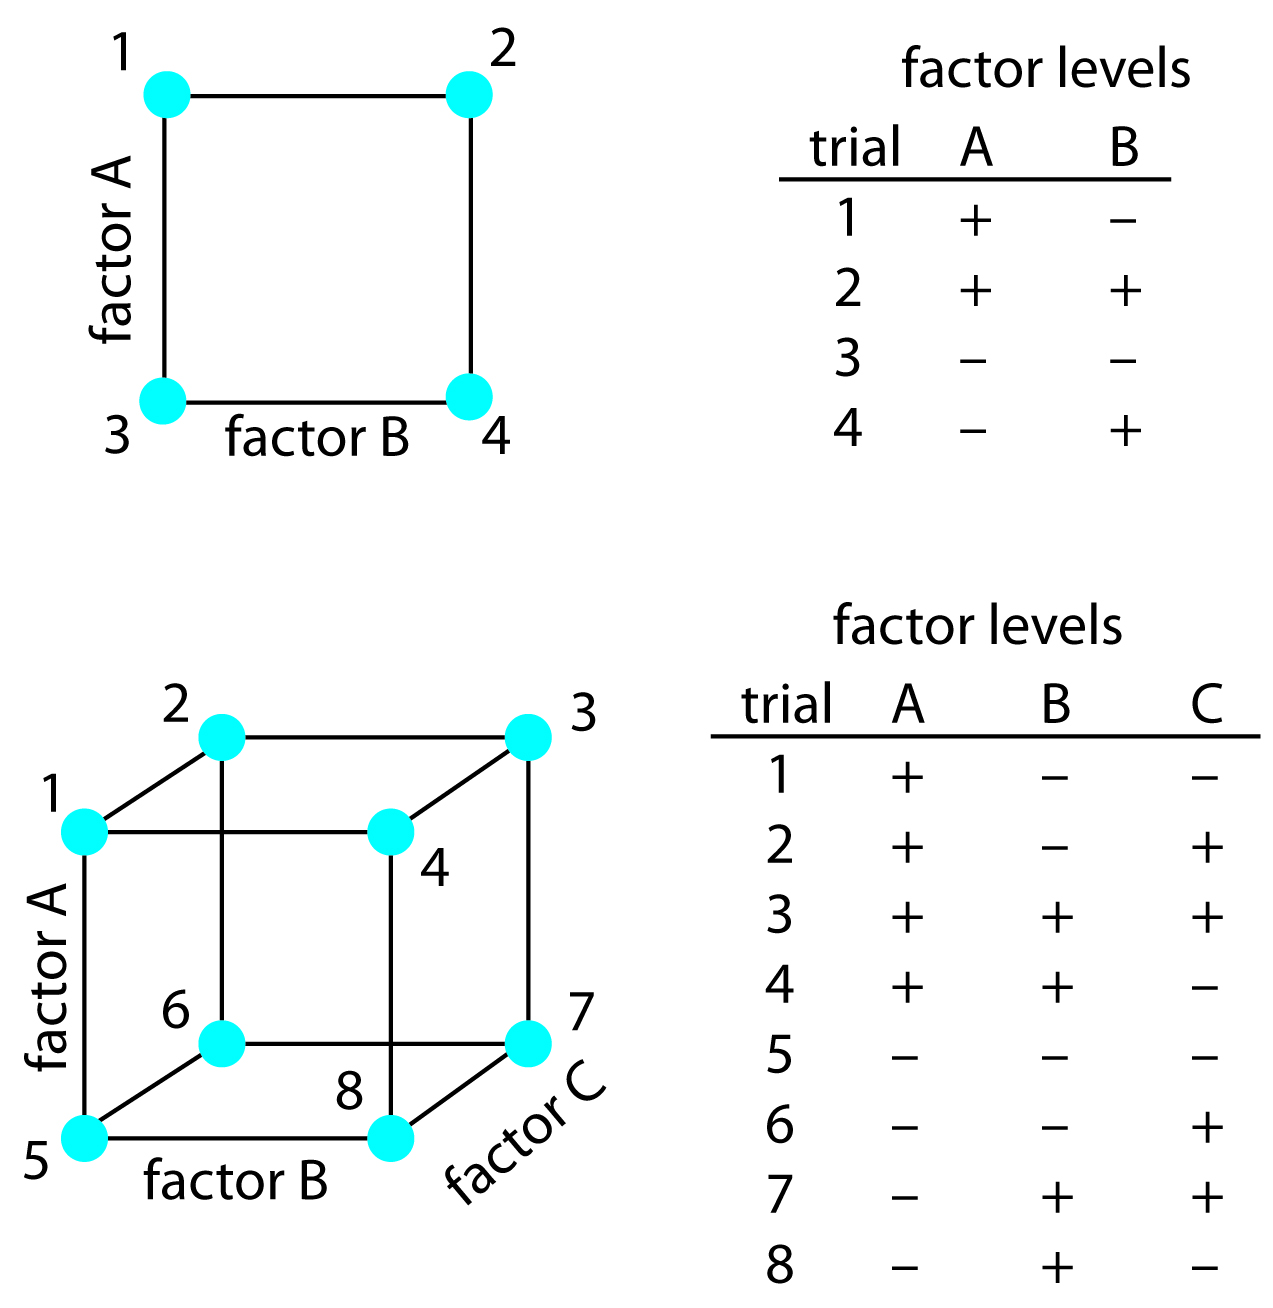
\includegraphics[width=0.7\linewidth, height=0.3\textheight]{art/full_factorial}
\caption[Full Factorial Design]{Full factorial designs: $2^2$ and $2^3$. \newline \url{http://chemwiki.ucdavis.edu/Analytical_Chemistry/Analytical_Chemistry_2.0/14_Developing_a_Standard_Method}}
\label{fig:full_factorial}
\end{figure}
With this $2^2$ design, we may recover several effects:
\begin{description}
\item [Main effect of A] The effect of varying $A$ from $(-)$ to $(+)$.
\item [Main effect of B] The effect of varying $B$ from $(-)$ to $(+)$.
\item [Main effects with interaction] The effect of varying both $A$ and $B$ from $AB=(--)$ to $AB=(++)$.
\end{description}



We typically denote the (mean) response for each treatment by the $\mu_{\smiley}$ notation, where $\smiley$ encodes the applied treatment by stating the conditions that were at their $+$ state:
\begin{table}[H]
\centering
\begin{tabular}{|c|c|c|c|}
\hline Treatment & A & B & Mean \\ 
\hline 1 & + & - & $\mu_a$ \\ 
\hline 2 & + & + & $\mu_{ab}$ \\ 
\hline 3 & - & - & $\mu_{(1)}$ \\ 
\hline 4 & - & + & $\mu_b$ \\ 
\hline 
\end{tabular} 
\end{table}

\marginnote{Interaction}

Slightly intruding into the realm of data analysis, a visualization of interactions is known as the \emph{interaction plot}, depicted in Figure~\ref{fig:interaction_plot}. 
The upper left panel demonstrates a lack of interaction (think why), while the upper right panel depicts an interaction.
\begin{figure}[ht]
\centering
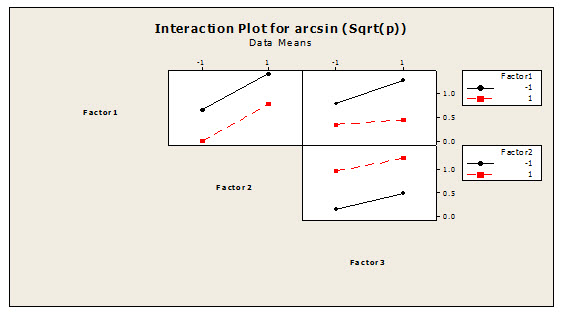
\includegraphics[width=0.3\textheight]{art/attribute_doe_interaction_plot}
\caption[Interactions plot]{Interactions plot. \newline \url{http://blog.minitab.com/blog/statistics-in-the-field/optimizing-attribute-responses-using-design-of-experiments-doe-part-2}}
\label{fig:interaction_plot}
\end{figure}


\begin{remark}[Popularity of $2^k$]
The $2^k$ designs are probably the most popular full factorial designs. 
This may be attributed to the fact that many factors studied really have two levels, but more plausibly, since these are merely \emph{screening} experiments. 
Once non related factors have been screened, the experimenter may proceed from the $2^k$ design to more elaborate ones. 
\end{remark}



\begin{remark}[Intermediate Factor Levels]
In a $2^k$ design, a factor may actually be a \textbf{continuous} controllable input which was restricted to two values for convenience. 
After estimating the effect of the factor, we may want to know what the effect would have been, had we set it on some intermediate level.
It is customary to assume that a main effect acts linearly in-between experimental conditions, yet you should remember that there is nothing in the data to support this.
For a more rigorous approach, see the Response Surface Methodology Section (\ref{sec:response_surface}).
\end{remark}





\subsubsection{$3^k$ Designs}
The name $3^k$ design is rather self explanatory.
If a continuous variable is discretized to $3$ levels, one may actually estimate and check for non-linear main-effects, which is impossible with $2^k$ designs. 
Then again, more than $2$ levels are rarely treated as full factorial experiments. 
This is because $3$ level factors typically appear when aiming at optimizing the factor level combination, for which the \emph{response surface} methodology of Section~\ref{sec:response_surface} is more economical.



\subsubsection{Full Factorial vs. One-Factor-at-a-Time}
Importantly, a factorial design is better than $k$ experiments with one factor at a time. This is because:
\begin{enumerate}
\item Factorial experiments make better (statistical) use of each sample unit for estimating main effects.
\item Factorial experiments allow the estimation of interactions between factors. 
\end{enumerate}
A classical illustration of the second point, is given in Figure~\ref{fig:one_factor_at_a_time}.
The figure depicts a one-factor-at-a-time optimization sequence (from A to H). Since the factors are not varied simultaneously, the experiments is unable to identify that the response is not a linear surface. 
Put differently, he is unable to estimate an interaction.

\begin{figure}[ht]
\centering
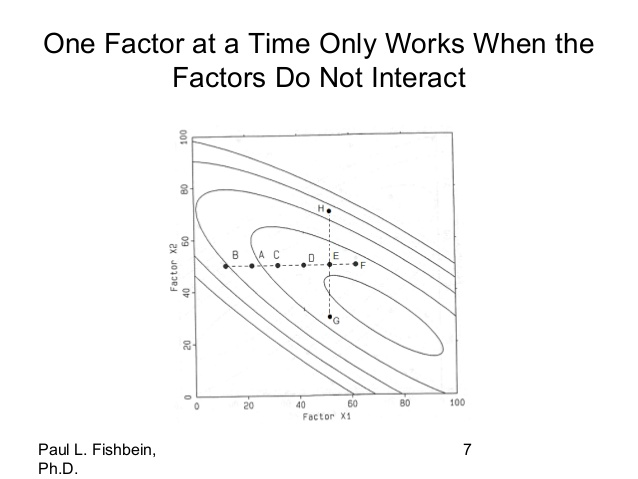
\includegraphics[height=0.3\textheight]{art/optimization-without-statistical-doe-2015-03-23-7-638}
\caption[One-at-a-time optimization]{Optimizing factors, one at a time.\newline \url{http://www.slideshare.net/PaulFishbein/optimization-without-statistical-doe-2015-03-23-46817073}}
\label{fig:one_factor_at_a_time}
\end{figure}





\subsection{Fractional Factorial}
Full factorial designs are the simplest designs to setup and interpret. 
A major drawback, are the resources required when $k$ is large. 
This is where the \emph{fractional factorial}, or \emph{partial factorial} designs kick in.
The fundamental idea is to design a full factorial, but skip a couple experimental conditions. If conditions to skip are wisely selected, only information on higher order interactions will be compromised.


\begin{example}[From $2^2$ to $2^{2-1}$]
\label{eg:fractional_factorial}
As a first toy example, we will try to save some time and money by eliminating particular conditions of the $2^2$ design in Figure~\ref{fig:full_factorial}.
As the name may suggest, a $2^{2-1}$ design, has $2$ experimental conditions in each run. 
There are thus $\binom{4}{2}=6$ possible eliminations, which are enumerated in Table~\ref{tab:partial_factorial} along with the extractable information in each elimination.
\begin{table}[ht]
\begin{tabular}{|p{2.5cm}|p{10cm}|}
\hline Elimination &  Problem \\ 
\hline
\hline 1,2 &  No information on $a$. \\ 
\hline 1,3 &  No information on $b$.\\ 
\hline 1,4 &  $a$ aliased with $b$ aliased with $ab$. \\ 
\hline 2,3 &  $a$ aliased with $b$ aliased with $ab$. \\ 
\hline 2,4 &  No information on $b$. \\ 
\hline 3,4 &  No information on $a$.\\ 
\hline 
\end{tabular} 
\caption[Aliasing]{Aliasing in a $2^{2-1}$ design: All possible eliminations from the $2^2$ design that lead to a $2^{2-1}$ design.}
\label{tab:partial_factorial}
\end{table}
\end{example}

The lesson from Example~\ref{eg:fractional_factorial} is that in a fractional factorial our savings in time and money, come at the cost of the information that can be drawn from the experiment.
The idea behind partial factorial experiments, is that by an informed choice of the conditions skipped, we can choose what information to give up. The information lost, is known as the \emph{alias structure}.\marginnote{Alias Structure}

In practice, we will rarely go over all the $\binom{2^k}{2^k-2^{k-p}}$ possible eliminations of conditions, but rather revert to pre-selected designs. 
Table~\ref{tab:partial_factorial_ii}, generated with the \rcode{FrF2()} in the \rcode{FrF2} \R package, is an optimal $2^{5-2}$ design.
Using the \rcode{design.info()} function of that same package, we know that the aliasing structure of this design is
$a=bd=ce, b=ad, c=ae, d=ab, e=ac$.
We will not go into the details of how the aliasing structure is computed, but rather refer the reader to \cite{cox_theory_2000}.
\begin{table}[ht]
\centering
\begin{tabular}{rrrrrr}
  \hline
 & A & B & C & D & E \\ 
  \hline
1 & -1 & 1 & -1 & -1 & 1 \\ 
  2 & 1 & -1 & 1 & -1 & 1 \\ 
  3 & -1 & -1 & -1 & 1 & 1 \\ 
  4 & -1 & 1 & 1 & -1 & -1 \\ 
  5 & -1 & -1 & 1 & 1 & -1 \\ 
  6 & 1 & 1 & 1 & 1 & 1 \\ 
  7 & 1 & -1 & -1 & -1 & -1 \\ 
  8 & 1 & 1 & -1 & 1 & -1 \\ 
   \hline
\end{tabular}
\caption[Fractional Factorial Design]{$2^{5-2}$ design.}
\label{tab:partial_factorial_ii}
\end{table}





\begin{extra}[Coding Theory]
There is a close relationship between design of experiments and coding theory in computer science. 
A possible reference on the matter is \cite{hill_first_1986}, or \cite{hedayat_orthogonal_1999}.
\end{extra}


%
%\subsection{Split Plot Design}
%\label{sec:split_plot}
%Revisiting our web site layout problem:
%We want to block along age and country. 
%For each age and country combination (full factorial blocking) we can randomly assign users to site layouts. 
%This combination of a factorial design for blocking, is known as a \emph{split plot}, or \emph{split unit} design.
%For more on split plots see \cite[Sec.6.4]{cox_theory_2000}.
%






%\section{Specialized blocking techniques}
%
%\subsubsection{Latin Square Design}
%[TODO: put section in context- variance? bias? economy?]
%When homogenous groups are defined by two non-specific factors, we would like to create blocks that are balanced, so that the non-specific factors do not bias effect estiamtes.
%In our running example, non-specific factors may be age and gender. 
%We could construct all age and gender combinations, and randomly assign users from each age-gender to each site design.
%This would is an example of a \emph{split plot} design, discussed in Section~\ref{sec:split_plot}.
%If, however, we do not deal with age-gender, but rather with age-country, we may not have enough users in each cell to assign to all site designs. 
%Since we do not want to estimate the effect of age, nor country, but merely balance the design so that age and country effects do not alias the site's effect, we do not actually need all age-country combinations. 
%
%
%
%If we have $k$ designs, we may group ages and countries into $k$ categories each, and each design is seen only once in each age group and once in each country group. 
%This allocation of treatment to blocks is known as a \emph{Latin Square}. 
%Table~\ref{tab:latin_square} demonstrates a Latin Square for $7$ web site designs, and compares it to a non-balanced allocation. 
%\begin{table}[ht]
%    \begin{minipage}{.5\linewidth}
%        \centering
%		\begin{tabular}{rlllllll}
%		  \hline
%		 & 1 & 2 & 3 & 4 & 5 & 6 & 7 \\ 
%		  \hline
%		1 & 1 & 2 & 3 & 4 & 5 & 6 & 7 \\ 
%		2 & 1 & 2 & 3 & 4 & 5 & 6 & 7 \\ 
%		3 & 1 & 2 & 3 & 4 & 5 & 6 & 7 \\ 
%		4 & 1 & 2 & 3 & 4 & 5 & 6 & 7 \\ 
%		5 & 1 & 2 & 3 & 4 & 5 & 6 & 7 \\ 
%		6 & 1 & 2 & 3 & 4 & 5 & 6 & 7 \\ 
%		7 & 1 & 2 & 3 & 4 & 5 & 6 & 7 \\ 
%		   \hline
%		\end{tabular}
%    \end{minipage}%
%    \begin{minipage}{.5\linewidth}
%      \centering
%		\begin{tabular}{rlllllll}
%		  \hline
%		 & 1 & 2 & 3 & 4 & 5 & 6 & 7 \\ 
%		  \hline
%		1 & 1 & 2 & 3 & 4 & 5 & 6 & 7 \\ 
%		  2 & 2 & 3 & 4 & 5 & 6 & 7 & 1 \\ 
%		  3 & 3 & 4 & 5 & 6 & 7 & 1 & 2 \\ 
%		  4 & 4 & 5 & 6 & 7 & 1 & 2 & 3 \\ 
%		  5 & 5 & 6 & 7 & 1 & 2 & 3 & 4 \\ 
%		  6 & 6 & 7 & 1 & 2 & 3 & 4 & 5 \\ 
%		  7 & 7 & 1 & 2 & 3 & 4 & 5 & 6 \\ 
%		   \hline
%		\end{tabular}
%		\end{minipage} 
%	\caption{A $7$-treatment, two-factor design. 
%	Left pane is not balanced.
%	Right pane is balanced with a Latin Square, generated with the \rcode{MOLS()} function of the \rcode{crossdes} \R package.}
%	\label{tab:latin_square}		
%\end{table}
%
%
%The following example makes the same point, with the original agricultural motivation for this design.
%\begin{example}[Agricultural Yield Study]
%\label{eg:latin_square}
%Consider an farmer growing corn.
%He wishes to study the effect of $7$ candidate fertilizers (single factor with $7$ levels).
%He is aware that the location of the plot may affect yield, due to slightly different sunlight, irrigation, altitude, etc.
%He thus assumes he has to deal with two extra variance sources: row and column of the plot. 
%He could treat the row and column as two factors, with $7$ levels each, be he does not care to estimate the row/column effect, but merely to avoid bias.
%He will thus try to look for an allocation of fertilizer to rows and columns so that any row/column effect will be averaged out.
%The Latin Square design of Table~\ref{tab:latin_square} does just that.
%\end{example}
%
%
%\begin{extra}\noindent
%\begin{enumerate}
%\item If the Latin Square reminds you of Soduko, it should. Soduko is just that!
%\item The Latin Square is a very economical design, and is not used as often as it should be.
%\item If we had reason to believe that different age groups in different countries respond differently to each site (an interaction), then the Latin Square may actually introduce aliasing. 
%\end{enumerate}
%\end{extra}
%
%
%
%\subsubsection{Extensions of the Latin Square}
%\begin{enumerate}
%\item \textbf{Latin Hypercube}: When balancing more than two non-specific factors, we will call upon \emph{latin hypercube designs}, \aka \emph{orthogonal latin squares}. \marginnote{Orthogonal Latin Squares}
%\item \textbf{Greco-Latin Square}: A latin-hypercube with three variability sources. 
%\end{enumerate}







\section{Continuous Factors}

If aiming at screening factors, the fact that a factor is continuous is immaterial. 
One may sample a continuous factor at two points, and treat it as a $2$ level factor.
This is not the case, however, if aiming at characterizing the full response surface, for which the factorial designs are no longer appropriate. 

When dealing with \emph{continuous factors}, or \emph{quantitative factors}, we have many more analysis strategies than when dealing with qualitative factors.


\subsection{Central Composite Design}
\label{sec:central_composite}

Clearly, we cannot identify non-linear factor effects when sampling a factor only at two levels.
We may thus opt for a full $3^k$ factorial design to fit a non-linear surface to the data.
The factor encoding would typically be $\{-1,0,1\}$,
A full $3^k$ factorial design may however be needlessly expensive, if many factor actually have linear effects.
A more common approach in industrial application is the \emph{central composite design}, where a $2^k$ design is augmented with well chosen sampling points. 
Unlike the previous factorial designs, this design is sequential: 
first screen the non-interacting factors, then augment the design for better estimation of the interactions and non-linearities. 
For more details see \cite[Sec.6.6]{cox_theory_2000}


\subsection{Response Surface Methodology}
\label{sec:response_surface}

As the name suggests, \emph{response surface methdology} deals with the estimation of the response surface to the levels of continuous factors.
The response surface methodology is similar to the Central Composite Design of Section~\ref{sec:central_composite}, except that it is aimed at finding an optimal combination of factor level, instead of estimating their effects. 








\section{An Industrial Emphasis}
The following approaches are particularly popular in industrial settings.

\subsection{Plackett-Burman design}
\label{sec:plackett_burman}

A \emph{Plackett-Burman Design} is a fractional factorial design optimized for \textbf{screening}. 
It is a very economical design when studying the \textbf{main effects} of a \textbf{large number} of factors. 



\subsection{Taguchi Methods}
\emph{Taguchi methods} is a collective name for the philosophy, design, and analysis methods in industrial applications promoted by Genichi Taguchi in 1970's Japan.
Focusing on the design principles, we summarize Taguchi's emphasis:

\begin{enumerate}

\item Achieving low variability is no-less important, and more challenging then achieving a target value. 
Log variability ($\log s$) is thus often used as the response.

\item Factors which can be controlled only in a lab, but not in production, are deliberately varied in the lab. 
%Typically with split plot designs (\ref{sec:split_plot}).

\item An ample use of Plackett–Burman designs (Section~\ref{sec:plackett_burman}), and its extensions, to screen large numbers of factors. 

\end{enumerate}





\section{Optimal Designs}

Our discussion until now has been informal with respect to the desirable qualities of a design. 
We used the idea of ``balance'' and ``orthogonality'' to avoid bias and unwelcome variability.
In this section, we try to formalize the notion of a ``good design''.
We start with some motivating examples.


\begin{example}[Design for linear regression]
\label{eg:design_linear}
Figure~\ref{fig:design_linear} demonstrates the effect of the different location of the sampling points ($x$) on the quality of the estimated regression line.
In a \textbf{linear} model, the figure depict and intuition suggests, that it is preferable to spread the sampling points as far as possible.
\begin{figure}[h]
\centering
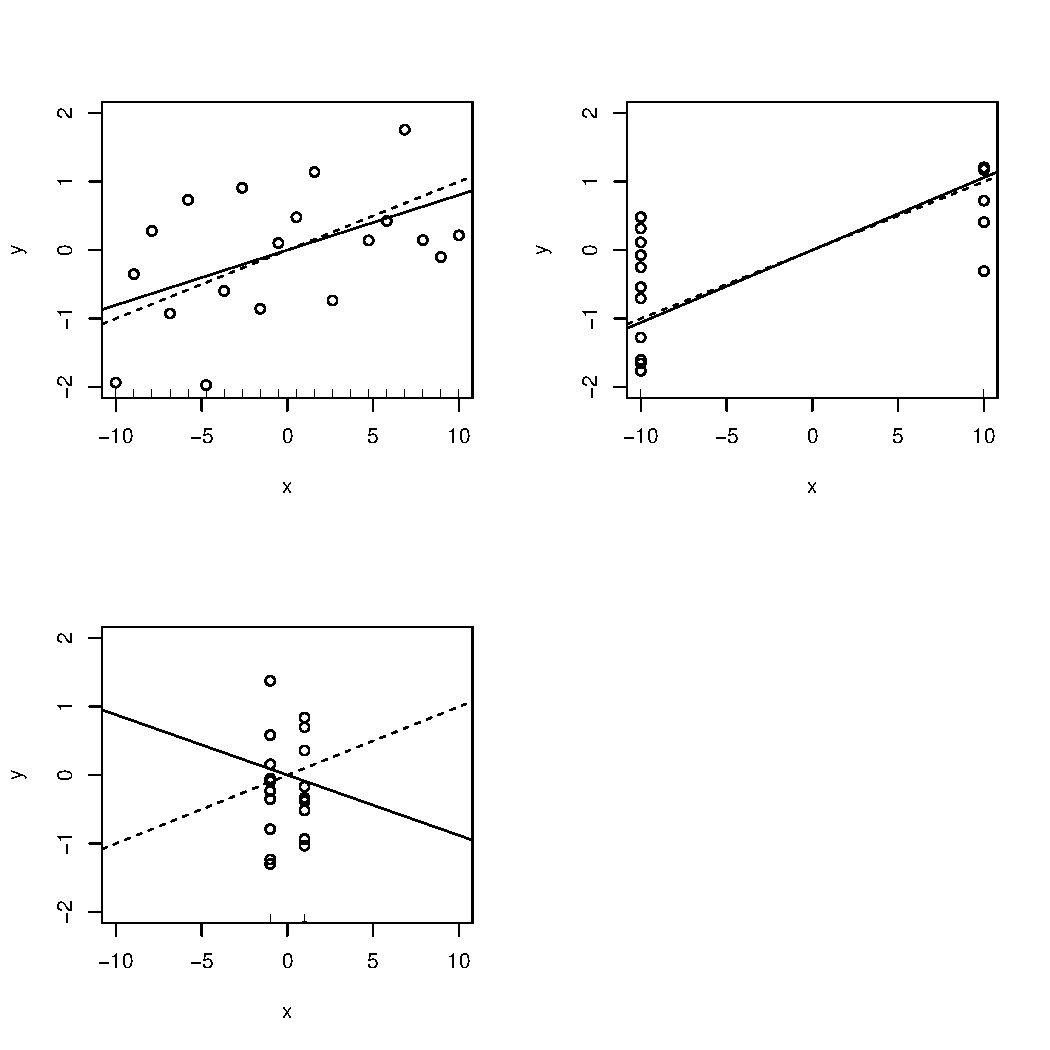
\includegraphics[height=0.3\textheight]{art/linear}
\caption[Design for Linear Models]{
Design for linear regression. Different panels show different designs. True function as a dashed line. Estimated function as a full line.}
\label{fig:design_linear}
\end{figure}
\end{example}





\begin{example}[Design for non linear regression]
\label{eg:design_non_linear}
Figure~\ref{fig:design_nonlinear} demonstrates the effect of the different location of the sampling points ($x$) on the quality of the estimated regression line, in a \textbf{nonlinear} model.
It may seems that unlike the linear case (Example~\ref{eg:design_linear}) optimality is achieved in some intermediate spread of the $x$s.
\begin{figure}[h]
\centering
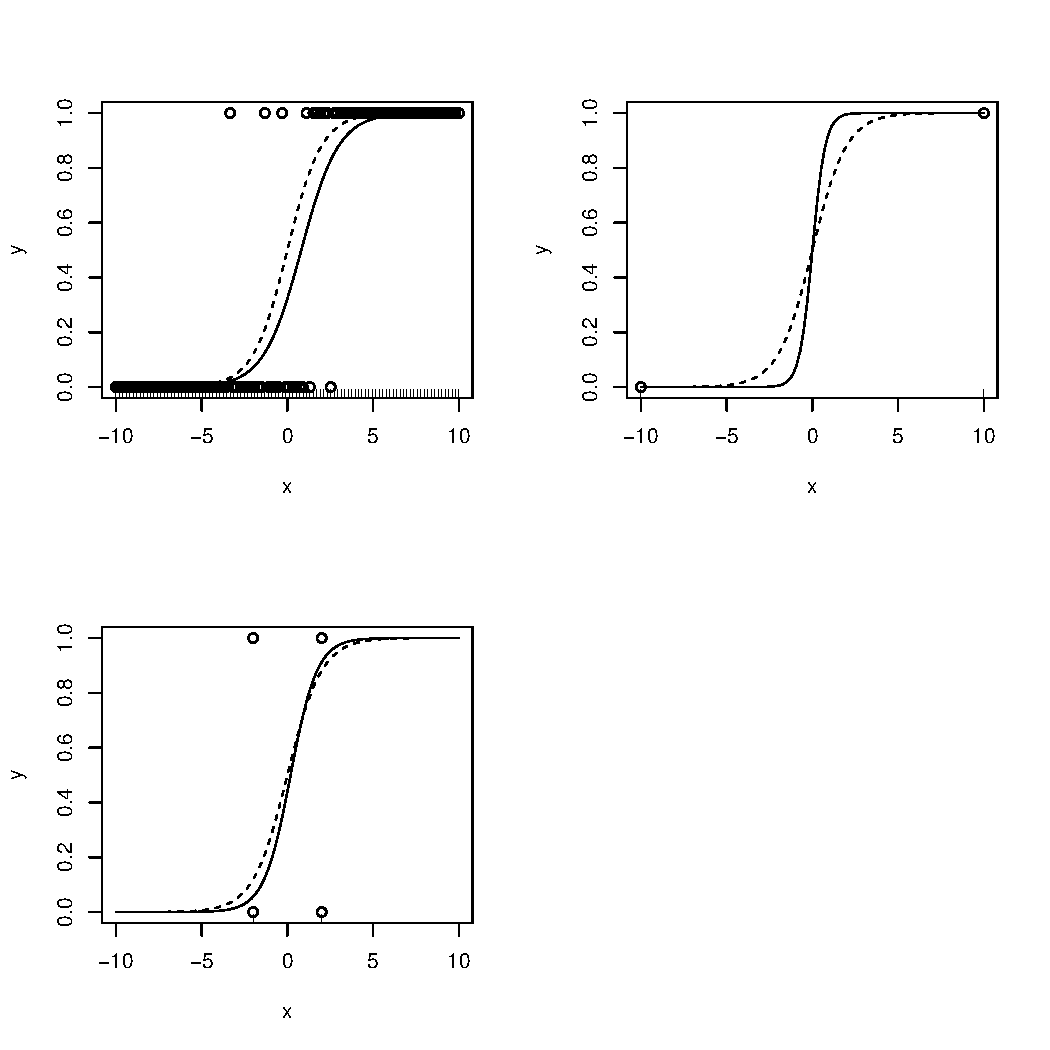
\includegraphics[height=0.3\textheight]{art/nonlinear}
\caption[Design for Non Linear Models]{Design for non linear regression. Different panels show different designs. True function as a dashed line. Estimated function as a full line.}
\label{fig:design_nonlinear}
\end{figure}
\end{example}





Now for some facts, supported by the previous examples:
\begin{enumerate}
\item The idea of ``balancing'' as a design criterion is very useful with discrete factors, but limited with continuous factors. 
\item For continuous factors with linear effects, the optimal design implies spreading the sampled factors levels as much as possible. 
\item For non-linear models, the optimal design may depend on the unknown true effects. 
\end{enumerate}



\subsection{Space Filling Design}
\label{sec:space_filling}
The most natural of designs, which is particularly suitable when we have no a-priori assumption on the functional relation ($f(x)$) between the (continuous) factors and the response, is known as a \emph{space filling design}.
As the name suggests, in a space filling design we aim at filling the factor space. Lacking any a-priori information, the filling will typically be as uniform as possible. 
We note however, that once information on $f(x)$ is made available, then a space filling design is typically sub optimal (see Example~\ref{eg:design_linear}).


\begin{extra}[Space Filling and Hashing]
If you are familiar with the idea of \emph{hashing functions}, then you may see the similarity between space filling and the \emph{uniformity} property of hash functions. 
For a more rigorous discussion, see \cite{hill_first_1986}.
\end{extra}



\subsection{Covariance Optimality}
When estimating the effect of a single continuous factor, we would like a design that gives us the most information per observation on some effect $\beta$. 
This is the same as minimizing the variance of the estimator, $\min \{Var[\hat{\beta}]\}$, with respect to the design.
In the case of linear regression with a single coefficient we know that 
\begin{align}
	Var[\hat{\beta}] &= \frac{\sigma^2_\varepsilon}{\sum_{i=1}^{n}(x_i-\bar{x})^2}.
\end{align}
Minimizing $Var[\hat{\beta}]$ is thus the same as spreading the $x$'s as far as possible, in accordance with the intuition from Example~\ref{eg:design_linear}.
Now recall that in a multivariate linear regression problem with an $n \times p$ design matrix, then 
\begin{align}
	Var[\hat{\beta}] &= \sigma^2_\varepsilon (X'X)^{-1}.
\end{align}
In this multivariate case, there may be several notions of ``maximal spread''. 
Denoting $M:= (X'X)^{-1}$, we can define:
\begin{definition}[A-Optimality]
	A design is said to be \emph{A-optimal} if it minimizes the average univariate variance.
	Formally: $\min \set{\Tr(M)}$.
\end{definition}
A-optimality does not account for covariances. 
In an extreme scenario, if we have several copies of the same variable, the more copies we have, the more importance that variable will be given by A-optimality.
The most popular optimality criterion is known as \emph{D-optimality}, and does not suffer from this phenomenon.
\begin{definition}[D-Optimality]
	A design is said to be \emph{D-optimal} if it minimizes the volume of the confidence region for $\beta$. 
	Formally: $\min \set{\det(M)}$.
\end{definition}

Both A-optimality and D-optimality implicitly target linear models, such as in Example~\ref{eg:design_linear}, because they aim at spreading the $x$'s. From Example~\ref{eg:design_non_linear} we know this to be sub-optimal for non-linear models. 
For non-linear designs, one may opt for space filing designs (\ref{sec:space_filling}), or consult \cite{pukelsheim_optimal_1993}. 



\begin{extra}[Other Optimality Criteria]
There are as many optimality criteria as there are matrix norms. For a more detailed review, see \cite{wikipedia_optimal_2015}.
For a mathematical rigorous, and through treatment, see \cite{pukelsheim_optimal_1993}.
\end{extra}







\section{Sequential Designs}
\label{sec:sequantial}
% Mark Vandelmeulenbruke

Consider a clinical trial with a treatment and control group.
Now assume the medicine being tested is a miracle cure with immediate improvement. 
Do we really need to keep administering placebos to the control group, just because that was the initial experimental design?
This is where sequential designs come in.
Interestingly, the initial application of a sequential design was not in drug testing, but rather in a military context \citep{wald_sequential_1945}.

The problem with sequential testing, is the \emph{type-I error inflation}, which is simply a \emph{multiplicity problem}. \marginnote{Multiplicity}
To see this, think about an endless sequential experiment. Also assume the null hypothesis is true. 
Because of consistency, then a regular (non sequential) experiment will not reject $H_0$?
But if the test is sequential, the type-I error of endlessly many tests at level $\alpha$ each, will certainly be making more than $\alpha$ mistakes (unless dependence is perfect).

In it simplest version, a sequential design allows early stopping for rejection of the null, or for futility (non-rejection). 
In more elaborate schemes then not only is early stopping allowed, but also the redesign of the experiment. 
This is known as \emph{adaptive design}. The crux, as usual, is not inflating the type-I error, or introducing bias, by redesigning.\marginnote{Adaptive Design}

We also remind the reader that we already met two sequential designs, aimed at estimating factor effects, and optimizing factor-level combinations.
These were the Central Composite Design (Section~\ref{sec:central_composite}) and Response Surface Methdology (Section~\ref{sec:response_surface}).

\begin{extra}[Active Learning]
In the machine learning literature, the idea of adaptive design of experiments is known as \emph{active learning}, where the emphasis is less on adaptive-testing, but rather on adaptive-estimation.
\end{extra}




\subsection{Pooled Designs}
\emph{Pooled designs}, \aka as \emph{group testing}, or \emph{hierarchical design}, appears when it is cheaper to measure the response for a group of experimental units simultaneously, rather then for each single one. 
It originated in the context of identifying soldiers with syphilis in WWII. It was the Harvard Economist Robert Dorfman that suggested that one may mix blood samples from several soldiers and then repeat the same in the subgroups that show the presence of syphilis \citep{dorfman_detection_1943}. 
The method became immensely popular in the DNA analysis age, where technology allows biologists to test for the presence of particular protein in a sample from a group of cells (e.g. a blood sample). 

Pooled designs broadly classify into two classes: 
\begin{description}
\item [Adaptive group testing] Where the groupings, and the groups to be tested depend on the previous results in the same experiment (see also \emph{adaptive designs}).
\item [Non-adaptive group testing] Where the experiment consists of sequential group tests, but the design is fixed independently of the experimental results. 
\end{description}


\begin{extra}[Bloom filters]
If you are familiar with data structures and particularly \emph{Bloom Filters}, then you will probably note that a Bloom filter is a data structure that groups objects in a way that facilitates lookup using group testing. 
\end{extra}



\section[AB testing]{$A\backslash B$ Testing}
Our web-site optimization example is interesting not only because it accommodates so many DOE practices, but it is also a practical problem of great interest.
For historical reasons, the experimentation with several web-site layouts is not called a factorial experiment (which it is), but rather an \emph{$A\backslash B$-test}.

Some particular characteristics of $A\backslash B$ testing include:
\begin{enumerate}
\item Users come by the millions. Sample size is rarely an issue, so that avoiding bias is more important than avoiding variability.
\item Browser cookies, or login details define blocks. Technology permits to optimize the size for each block separately. If blocking is to very specific subgroups (female users, running Linux, that purchased on Amazon, etc.), then sample size, and thus variability, may become an issue again.
\item Sites have many layout parameters (locations, colours, sizes,...). Studying all these combinations may result on a formidable task (full factorial?!?).
\end{enumerate}




\section{Computer Experiments}
% no randomness
% space filling parameter choices for simulation
\begin{example}[Designing Wings]
\label{eg:wings}
Consider the problem of designing an air-craft's wing.
We would like to know how the wing's attributes, i.e., factors, govern its lift.
We could obviously conduct real-life experiments by varying the wing's attributes, building the wing, flying the air-plane, and recording results. 
Needless to say how expensive this process is.
It is much more reasonable to program the differential equations that govern the lift to a computer, fix several factors values, and solve the equations.
This is what \emph{computer experiments} are all about. 
\end{example}


The wind design example (\ref{eg:wings}) demonstrates the following points:
\begin{enumerate}
\item Computer experiments are essentially numerical solutions to complicated systems of equations.
\item Because solutions take a lot of time, only a small finite set of factor levels may be evaluated. 
\item The ``response'' to each treatment, is deterministic. 
\item The problem of interest is in reconstructing the response at non measured factor levels, so that optimal values may be identified. 
\end{enumerate}
It is thus not uncommon to call upon DOE theory for choosing the factor combinations to be experimented with. Space filling designs (Sec.~\ref{sec:space_filling}) being a particularly prevalent choice. 
The analysis of computer experiment is very different than real-life experiment since we have no noise component. 
See \cite{sacks_design_1989} or \cite{santner_design_2013} for further details. 



\section{Observational Studies}
\label{sec:observational}

In this section we abandon controlled experiments, in which we were able to randomize, and choose the factors levels to be measured.
In observational studies, we have no such controls. 
As such, there are no \emph{factors}, but rather, only covariates. 


\begin{example}[Post-sale testing]
	\label{ex:post-sale}
	Consider the notorious Galaxy Note7, or any car, plane, smartphone, or software. 
	Bug malfunctions will always be found after launch.
	One way to discover what triggers the malfunction is to replicate it under a designed experiment. 
	A possibly better way is to collect failure data post-sale.
	This is why your software asks you to send crash reports. 
	This is why plane and engine manufacturers equip top engines with sensors and communications, to be transmitted constantly. 	
\end{example}


Observational studies classify into:
\begin{description}
	\item[Cross Sectional] Where each sample unit, i.e. individual, is observed in a single point in time. 
	\item[Prospective] Where each sample unit is observed on various occasions in the future. 
	\item[Retrospective] Where measurements are recovered on sample units from the past, based on some outcome. 
\end{description}


Being the simplest type of observational study, there really not much to say about \emph{cross sectional} studies, except a vivid warning against causal inference from such studies (see \ref{sec:causal}).

In \emph{prospective studies}, \aka \emph{longitudinal data}, or \emph{cohort study}, sampling units are selected and then measured over time alongside covariates. \marginnote{Longitudinal Data}

For the study of rare outcomes, prospective studies may be very wasteful. 
Retrospective studies, \aka \emph{case-control studies} remedy this by collecting units with the desired outcome, and only then matching them with controls and recovering their event history. In the words of \cite{cox_principles_2011}: {\em \dots a prospective study looks for the effects of causes whereas a retrospective study examines the causes of effects}.\marginnote{Case-Control Study}
This is clearly not a random sample in the population, so it is unclear that inference in retrospective studies is valid. 

To demonstrate the difference between the sampling schemes consider a binary outcome $Y\in\set{0,1}$ and a binary covariate $X\in\set{0,1}$. 
In terms of the post-sale problem in Example~\ref{ex:post-sale}, $X$ can stand a version indicator, and $Y$ a failure indicator. 
The effect of $X$ on $Y$, can be quantified by the \emph{odds ratio}. 
To define the odds ratio, we first define the \emph{odds}.

\begin{definition}[Odds]
	The odds of two events, $Y=1$, and $Y=0$, is defined as 
	\begin{align}
	Odds:= P(Y=1)/P(Y=0).
	\end{align}
\end{definition}
The \emph{odds}, just like \emph{probabilities} is an uncertainty measure. 
It quantifies the ratio of ``successes'' per ``fail''. 
In some communities, the odds are actually more popular than probabilities (think horse racing).
In our post-sale example, the odds measures the ratio of working devices per faulty device (not per \emph{produced} device like the probability measure). 



The odds ratio is the ratio of odds under two conditions: 
\begin{definition}[Odds Ratio]
	\begin{align}
	OR := \frac{P(Y=1|X=1) / P(Y=0|X=1)}{P(Y=1|X=0) / P(Y=0|X=0)}.
	\end{align}
\end{definition}
Just in order to emphasize what the OR is \textbf{not}, we also define the \emph{relative risk}, which is perhaps a more natural effect measure:
\begin{definition}[Relative Risk]
	\begin{align}
	RR := \frac{P(Y=1|X=1)}{P(Y=1|X=0)}.
	\end{align}
\end{definition}
You may not verify that if $X$ has not effect on $Y$, then both $OR=1$ and $RR=1$. 
We now show how the $OR$ can be estimated from the various studies designs. 


\paragraph{Prospective Study} 
A prospective study means that we decide how many samples of each version to take and wait until some fail, and then compare the failure probabilities. 
Formally this means we can estimate $P(Y=1|X=1)$ and $P(Y=1|X=0)$.
Estimating $OR$ is trivial is thus trivial.


\paragraph{Retrospective Study}
A retrospective study means that we sample a fixed number of working or broken devices. 
We can thus estimate the frequency of each version given the outcome: $P(X|Y)$.
To relate it to the $OR$, we will need to relate the estimable $P(X|Y)$, to the desired $P(Y|X)$ via Bayes' Theorem: 
\begin{align}
\label{eq:bayes}
	P(Y|X)=P(X|Y)P(Y)/P(X)
\end{align}

Several applications of Eq.(~\ref{eq:bayes}) yields that 
\begin{align}
\label{eq:retrospective_OR}
	OR 	&= \frac{P(X=1|Y=1)/P(X=1|Y=0)}{P(X=0|Y=1)/P(X=0|Y=0)}.
\end{align}
Eq.(\ref{eq:retrospective_OR}) is very good news. 
It means that we even if we sample retrospectively, we can estimate the OR as if we sampled prospectively. 

\begin{think}
	Can we estimate other effect measures such as the RR from a retrospective study?
\end{think}



\paragraph{Cross-Section}
A cross-section study is not a probable sampling scheme for our post-purchase analysis. 
It implies that we sample randomly in a ``pile'' of devices of all versions and states. 
We thus get an estimate of the proportion of each $X,Y$ combination, and need to relate it to the difference in failure probabilities. 
Formally, we estimate all $P(Y,X)$'s, which for brevity we denote $\pi_{yx}$.
For example $\pi_{00}$ for $P(Y=0,X=0)$ etc. 
Via Bayes' Theorem we then have 
\begin{align*}
	OR = \frac{\pi_{11}\pi_{00}}{\pi_{10}\pi_{01}},
\end{align*}
we shows that the OR can also be estimated from a cross-section study.

\begin{think}
	Can you estimate the RR from a cross section study?
\end{think}


\begin{think}
	In regression analysis we typically analyze bias and variance while conditioning on the design matrix, $X$. 
	Is such a practice consistent with the designed experiment or the observational view of a study?
	If observational, is it cross sectional? Prospective? Retrospective? 
\end{think}





\subsection{Causal Inference}
\label{sec:causal}

Causal inference is typically the Holy-Grail of empirical research. 
Causality may be inferred from a designed experiment, or from an observational study. 
As already stated on several occasions, inferring causality from observational studies is much riskier than from designed experiments. 
This is because in observational studies we have two sources of uncertainty, that are canceled by the randomization mechanism of designed experiments. 
This first is the existence of non-controlled variables, that affect both ####







\section{Bibliographic Notes}
Our general discussion of observational studies, designed experiments, causal inference, etc, is derived from \cite{cox_principles_2011}.
For an overview of DOE see \cite{cox_theory_2000}, \cite{mason_statistical_2003}, \cite{everitt_cambridge_2010}. 
Another nice and freely available resource is a Penn State course on the topic\footnote{\url{https://onlinecourses.science.psu.edu/stat503/node/1}}. 
Some seminal references in the field include \cite{fisher_design_1960} and \cite{box_statistics_1978}.
For respondent driven sampling see \cite{berchenko_modeling_2013}.
For causal inference in non-designed experiments see \cite{rosenbaum_observational_2002}. 
For optimal designs see \cite{pukelsheim_optimal_1993}.
For analysis of data: linear models, ANOVA, etc.\ there are endlessly many books. This author's recommendations include \cite{hocking_analysis_1985}, \cite{greene_econometric_2003}. 
For the relation between factorial designs and coding theory in computer science, see \cite{hill_first_1986}. 
For design and analysis of computer experiments, see \cite{sacks_design_1989} or \cite{santner_design_2013}.
